\chapter{TINJAUAN PUSTAKA}
\label{chap:tinjauanpustaka}

\section{Hasil Penelitian Terdahulu}
\label{sec:hasilpenelitianterdahulu}

Sejumlah penelitian mengenai segmentasi visual telah dilakukan, di antaranya oleh \textcite{Dharma2025PerformanceEvaluation} dan \textcite{wang2023internimage}.
Penelitian \textcite{Dharma2025PerformanceEvaluation} menjelaskan bahwa performa \emph{DeepLabV3 Plus} dengan \emph{backbone} ResNet-50 yang dilatih dengan \emph{dataset} lokal ITS pada malam hari mendapatkan performa paling baik mencapai \emph{mean Intersection over Union} (mIoU) 76,45\% dan \emph{Pixel Accuracy} 99,64\% pada kelas jalan.
Sementara itu, penelitian \textcite{wang2023internimage} mengusulkan \emph{InternImage} sebagai \emph{backbone} segmentasi berbasis \emph{Deformable Convolution v3} (DCNv3) yang dipralatih dengan \emph{dataset} global Mapillary Vistas dan dilakukan proses \emph{fine-tuning} pada \emph{dataset} global Cityscapes, mendapatkan mIoU yang lebih tinggi yaitu 87,0\% pada \emph{dataset} validasi Cityscapes.
Terdapat juga penelitian yang berfokus pada optimalisasi model \emph{deep-learning} sehingga model dapat berjalan secara \emph{real-time} pada komputer kendaraan.
Penelitian itu di antaranya adalah penelitian \textcite{zhou2022exploring} yang menunjukkan bahwa \emph{TensorRT} mampu mempercepat \emph{inference} model hingga 1,6-2 kali lipat melalui teknik \emph{layer fusion} dan optimalisasi memori, serta hingga 3,7 kali lipat dengan kuantisasi INT8 tanpa penurunan akurasi yang signifikan.
Perbandingan penelitian segmentasi visual tersebut disajikan pada Tabel \ref{tab:perbandingan_terdahulu}.

\begin{table}[H]
  \centering
  \caption{Perbandingan penelitian segmentasi visual}
  \label{tab:perbandingan_terdahulu}
  \renewcommand{\arraystretch}{1.4}
  \begin{tabular}{p{2.5cm}cc}
    \hline
    \textbf{Parameter} & \textbf{(Dharma et al., 2025)} & \textbf{(Wang et al., 2023)} \\
    \hline
    Arsitektur & DeepLabV3+ & InternImage (DCNv3) \\
    \emph{Dataset} & ITS lokal (malam) & Mapillary + Cityscapes \\
    mIoU & 76,45\% & 87,0\% \\
    Navigasi & Tidak & Tidak \\
    \hline
  \end{tabular}
\end{table}

Penelitian yang membahas lokalisasi dan perencanaan trajektori juga telah dilakukan, di antaranya oleh \textcite{Zazuli2024SensorFusion} dan \textcite{Philion2020LSS}.
Hasil penelitian \textcite{Zazuli2024SensorFusion} mendapatkan rata-rata galat 0,43 m pada laju kontrol 50 Hz dengan menggabungkan data sensor GNSS, odometri roda, dan IMU dengan metode \emph{Extended Kalman Filter} (EKF).
Sistem lokalisasi ini masih mengandalkan GPS sebagai acuan utama, sehingga ketika sinyal GPS terganggu, sistem tidak memiliki mekanisme untuk tetap bernavigasi.
Sementara itu, penelitian \emph{trajectory sampling} dari \emph{Lift, Splat, Shoot} (LSS) oleh \textcite{Philion2020LSS} memperkenalkan mekanisme \emph{shooting} trajektori pada representasi \emph{Bird's Eye View} (BEV) yang memungkinkan pemilihan trajektori berdasarkan \emph{cost} terendah.


\section{Dasar Teori}
\label{sec:dasarteori}

\subsection{Segmentasi Semantik Visual dan Optimasi \emph{TensorRT}}
\label{subsec:segmentasi-semantik}

Segmentasi semantik visual merupakan proses klasifikasi setiap piksel pada citra ke dalam kelas tertentu, yang dalam konteks kendaraan otonom digunakan untuk mengenali area jalan yang dapat dilalui \parencite{wang2023internimage}.
Berbeda dengan \emph{instance segmentation} yang membedakan objek individu, segmentasi semantik memberikan label pixel tanpa peduli informasi objek, sehingga lebih fokus pada pemahaman area jalan secara keseluruhan.
Perbedaan ini ditunjukkan pada Gambar \ref{fig:segmentasi_visual} di mana semua piksel dilabeli berdasarkan kelasnya.

\begin{figure}[H]
  \centering
  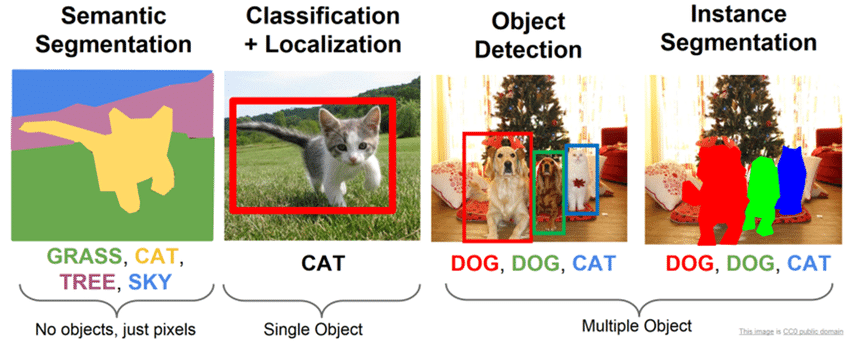
\includegraphics[width=0.8\textwidth]{gambar/semantic_vs_other.png}
  \caption{Perbandingan segmentasi semantik, klasifikasi dan lokalisasi, deteksi objek, dan \emph{instance segmentation} \parencite{Jaikumar2022MaskRCNN}}
  \label{fig:segmentasi_visual}
\end{figure}

InternImage merupakan salah satu arsitektur \emph{backbone} segmentasi dengan \emph{Deformable Convolution v3} (DCNv3) yang memiliki keunggulan dalam mengatasi keterbatasan konvolusi reguler \parencite{wang2023internimage}.
Tidak seperti pada konvolusi tradisional yang mengambil sampel piksel pada grid yang tetap, \emph{Deformable Convolution} mampu melakukan sampling piksel secara adaptif mengikuti bentuk objek pada citra seperti yang ditunjukkan pada Gambar \ref{fig:dcn}.
Kemampuan ini sangat berguna pada bentuk jalan yang beragam, seperti tikungan atau persimpangan, sehingga model dapat mengenali area jalan dengan lebih akurat.
Model ini menempati peringkat pertama di antara model \emph{open-source} segmentasi pada \emph{benchmark} Cityscapes pada kategori mIoU \emph{class}.


\begin{figure}[H]
  \centering
  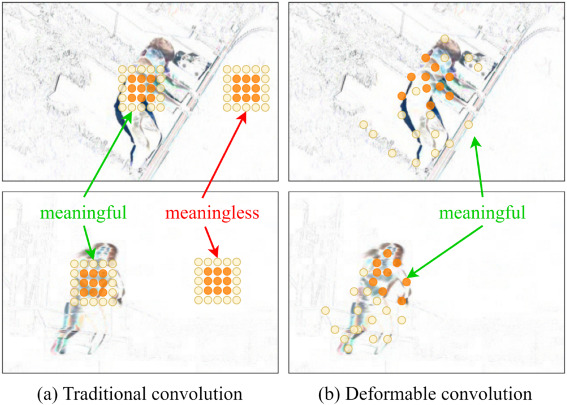
\includegraphics[width=0.57\textwidth]{gambar/traditional_conv_vs_dcn.jpg}
  \caption{Perbandingan konvolusi tradisional dan Deformable Convolution \parencite{MOU2025130770}}
  \label{fig:dcn}
\end{figure}

\emph{TensorRT} merupakan \emph{platform} optimasi \emph{inference} dari NVIDIA yang mempercepat eksekusi model \emph{deep learning} melalui dua teknik utama.
Pertama, \emph{layer fusion} menggabungkan beberapa \emph{layer} yang berurutan menjadi satu operasi komputasi GPU, sehingga mengurangi \emph{overhead} pembacaan dan penulisan data antar \emph{layer} \parencite{zhou2022exploring}.
Kedua, kuantisasi presisi ke \emph{half-precision floating-point} (FP16) mengurangi ukuran bobot model dari 32-bit menjadi 16-bit per parameter.
Berbeda dengan kuantisasi INT8 yang memerlukan kalibrasi, FP16 tidak memerlukan \emph{dataset} kalibrasi dan mempertahankan akurasi yang sangat dekat dengan presisi penuh \parencite{zhou2022exploring}.
Kombinasi kedua teknik ini memungkinkan model segmentasi yang berukuran besar untuk dijalankan secara \emph{real-time} pada GPU kendaraan.

\subsection{Kalibrasi Kamera dan Transformasi \emph{Bird's Eye View}}
\label{subsec:bev}

\emph{Bird's Eye View} (BEV) merupakan representasi pandangan atas (\emph{top-down view}) yang mempertahankan proporsi jarak dan sudut sebenarnya pada bidang jalan.
Transformasi dari citra kamera ke BEV pada penelitian ini menggunakan model kalibrasi kamera \emph{omnidirectional} yang dikembangkan oleh \textcite{Scaramuzza2006ICVS}.
Metode ini memodelkan fungsi proyeksi kamera sebagai deret Taylor pada persamaan \eqref{eq:scaramuzza_taylor}.

\begin{equation}
  f(\rho) = a_0 + a_1 \rho + a_2 \rho^2 + \ldots + a_N \rho^N,
  \label{eq:scaramuzza_taylor}
\end{equation}

Variabel $\rho$ adalah jarak radial dari pusat distorsi dan $a_0, a_1, \ldots, a_N$ adalah koefisien polinomial yang diperoleh dari proses kalibrasi menggunakan pola papan catur pada beberapa orientasi berbeda yang ditunjukkan pada Gambar \ref{fig:calibration}.
Parameter kalibrasi kemudian digunakan untuk membangun \emph{remap maps} yang memetakan setiap piksel pada citra BEV ke piksel yang bersesuaian pada citra kamera asli seperti yang ditunjukkan pada Gambar \ref{fig:construction}.

\begin{figure}[H]
  \centering
  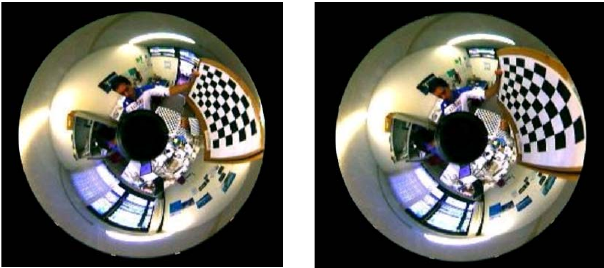
\includegraphics[width=1\textwidth]{gambar/chessboard_orientation.png}
  \caption{Proses kalibrasi kamera omnidirectional menggunakan pola papan catur \parencite{Scaramuzza2006ICVS}}
  \label{fig:calibration}
\end{figure}

\begin{figure}[H]
  \centering
  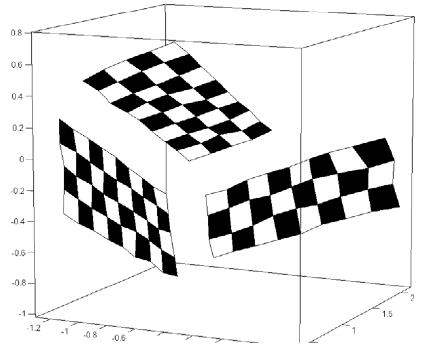
\includegraphics[width=0.6\textwidth]{gambar/konstruksi_3d.png}
  \caption{Hasil gambar yang telah direkonstruksi ulang ke dalam bentuk 3D menggunakan parameter kalibrasi \parencite{Scaramuzza2006ICVS}}
  \label{fig:construction}
\end{figure}

\subsection{Sensor Fusion dengan \emph{Kalman Filter}}
\label{subsec:kalman-filter}

\emph{Kalman Filter} merupakan estimator rekursif yang mampu memperkirakan \emph{state} dari suatu sistem berdasarkan pengukuran yang mengandung \emph{noise}.
Secara garis besar, Kalman Filter bekerja dalam dua tahap yaitu tahap prediksi (\emph{State Extrapolation Equation}) dan tahap koreksi (\emph{State Update Equation}).
Tahap prediksi merupakan proses proyeksi \emph{state} sekarang ke langkah waktu berikutnya menggunakan model sistem.
Sedangkan tahap koreksi merupakan proses memperbarui hasil prediksi dengan data pengukuran aktual \parencite{Becker2024KF}.
Kedua tahap ini dilakukan berulang membentuk siklus prediksi-koreksi secara terus-menerus yang ditampilkan pada Gambar \ref{fig:kalman_works}.

\begin{figure}[H]
  \centering
  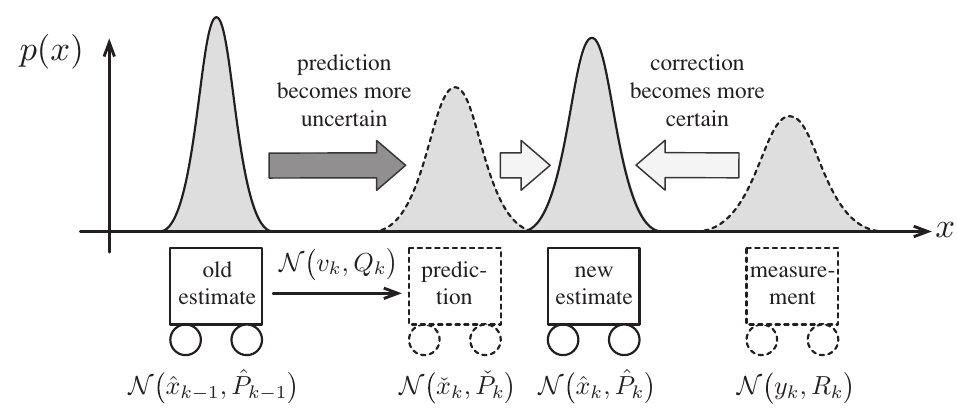
\includegraphics[width=0.8\textwidth]{gambar/kalman_works.png}
  \caption{Siklus prediksi dan koreksi Kalman Filter \parencite{Barfoot2017}}
  \label{fig:kalman_works}
\end{figure}

Untuk menerapkan siklus prediksi-koreksi tersebut, diperlukan model sistem yang mampu mendeskripsikan dinamika \emph{state} yang akan diestimasi.
Model \emph{state} yang digunakan pada penelitian ini adalah vektor posisi-kecepatan dalam kerangka koordinat lokal.

\textbf{Tahap Prediksi.} Prediksi \emph{state} dilakukan menggunakan persamaan berikut:

\begin{equation}
  \hat{\mathbf{x}}_k^- = \mathbf{A} \hat{\mathbf{x}}_{k-1} + \mathbf{B} u_{k-1},
  \label{eq:kf_predict_x}
\end{equation}
\begin{equation}
  \mathbf{P}_k^- = \mathbf{A} \mathbf{P}_{k-1} \mathbf{A}^\top + \mathbf{Q},
  \label{eq:kf_predict_p}
\end{equation}

Pada persamaan \eqref{eq:kf_predict_x}, $\mathbf{A}$ merupakan matriks transisi sistem yang memproyeksikan \emph{state} dari langkah waktu sebelumnya ke langkah waktu sekarang, $\mathbf{B}$ merupakan matriks masukan yang memetakan pengaruh vektor masukan terhadap perubahan \emph{state}, $\hat{\mathbf{x}}_k^-$ adalah \emph{state} hasil prediksi (\emph{priori}), $\hat{\mathbf{x}}_{k-1}$ adalah \emph{state} koreksi sebelumnya (\emph{posteriori}), dan $u_{k-1}$ adalah vektor masukan dari sensor inersia.
Persamaan \eqref{eq:kf_predict_p} disebut \emph{Covariance Extrapolation Equation}, di mana $\mathbf{P}_k^-$ merupakan kovarians estimasi \emph{priori}, $\mathbf{P}_{k-1}$ merupakan kovarians estimasi sebelumnya, dan $\mathbf{Q}$ merupakan kovarians \emph{process noise} yang mewakili ketidakpastian model sistem. Kovarians selalu ikut dipropagasi karena Kalman Filter memperlakukan \emph{state} sebagai variabel acak berdistribusi normal \parencite{Becker2024KF}.
Diskritisasi sistem kontinu ke diskrit dilakukan menggunakan metode \emph{matrix exponential} sebagaimana dijelaskan oleh \textcite{Dahdah2025}.

\textbf{Tahap Koreksi.} Setelah prediksi diperoleh, Kalman Filter menghitung selisih antara pengukuran aktual dengan prediksi. Selisih ini disebut \emph{innovation} atau \emph{residual} yang ditunjukkan pada suku $(\mathbf{z}_k - \mathbf{C} \hat{\mathbf{x}}_k^-)$ di persamaan \eqref{eq:kf_update} \parencite{Barfoot2017}. \emph{Innovation} kemudian diberi bobot oleh \emph{Kalman Gain} dan ditambahkan ke prediksi:

\begin{equation}
  \mathbf{K}_k = \mathbf{P}_k^- \mathbf{C}^\top (\mathbf{C} \mathbf{P}_k^- \mathbf{C}^\top + \mathbf{R})^{-1},
  \label{eq:kf_gain}
\end{equation}
\begin{equation}
  \hat{\mathbf{x}}_k = \hat{\mathbf{x}}_k^- + \mathbf{K}_k (\mathbf{z}_k - \mathbf{C} \hat{\mathbf{x}}_k^-),
  \label{eq:kf_update}
\end{equation}

Pada persamaan tersebut, $\mathbf{z}_k$ merupakan vektor pengukuran dari sensor, $\mathbf{C}$ merupakan matriks observasi yang memetakan \emph{state} ke ruang pengukuran, $\mathbf{R}$ merupakan kovarians \emph{measurement noise}, dan $\mathbf{K}_k$ merupakan \emph{Kalman Gain}.

\emph{Kalman Gain} ($\mathbf{K}$) merupakan inti dari Kalman Filter.
Nilai $\mathbf{K}_k$ dihitung ulang pada setiap iterasi berdasarkan $\mathbf{P}_k^-$ dan $\mathbf{R}$ \parencite{Becker2024KF}.
Jika $\mathbf{R}$ kecil (pengukuran akurat), $\mathbf{K}_k$ membesar sehingga estimasi lebih bergantung pada pengukuran.
Sebaliknya, jika $\mathbf{P}_k^-$ kecil (prediksi akurat), $\mathbf{K}_k$ mengecil sehingga estimasi lebih bergantung pada prediksi.
Hal inilah yang membedakan Kalman Filter dari \emph{A-B filter} yang memiliki \emph{gain} tetap.
Kalman Filter bersifat adaptif terhadap perubahan kualitas data secara \emph{real-time} \parencite{Becker2024KF}.

Setelah \emph{state} diperbarui, kovarians estimasi juga harus diperbarui. Bentuk paling sederhana dari pembaruan kovarians adalah:

\begin{equation}
  \mathbf{P}_k = (\mathbf{I} - \mathbf{K}_k \mathbf{C}) \mathbf{P}_k^-,
  \label{eq:kf_cov_simple}
\end{equation}

Meskipun lebih ringkas, bentuk \eqref{eq:kf_cov_simple} rentan kehilangan sifat simetris dan \emph{positive semi-definite} akibat pembulatan numerik \emph{floating-point} sehingga dapat menyebabkan divergensi filter. Untuk mengatasi hal ini, Barfoot merekomendasikan \emph{Joseph stabilized form} \parencite{Barfoot2017}:

\begin{equation}
  \mathbf{P}_k = (\mathbf{I} - \mathbf{K}_k \mathbf{C}) \mathbf{P}_k^- (\mathbf{I} - \mathbf{K}_k \mathbf{C})^\top + \mathbf{K}_k \mathbf{R} \mathbf{K}_k^\top,
  \label{eq:kf_cov_update}
\end{equation}

Pada persamaan tersebut, $\mathbf{I}$ merupakan matriks identitas. Bentuk Joseph menjamin $\mathbf{P}_k$ tetap simetris dan \emph{positive semi-definite} selama $\mathbf{R}$ \emph{positive semi-definite}, sehingga mencegah divergensi numerik pada implementasi \parencite{Barfoot2017}.

\subsection{\emph{Bicycle Model} dan Kinematika Kendaraan}
\label{subsec:bicycle-model}

\emph{Bicycle model} merupakan penyederhanaan model kendaraan \emph{Ackermann} empat roda menjadi model dua roda, di mana sepasang roda depan digabung menjadi satu roda kemudi dan sepasang roda belakang digabung menjadi satu roda penggerak \parencite{BouGhosn2024ITSC}. Model ini mengasumsikan tidak ada \emph{slip} pada kedua roda dan mengabaikan dinamika \emph{pitch} dan \emph{roll}. Persamaan kinematika \emph{bicycle model} dinyatakan sebagai:

\begin{equation}
  \begin{aligned}
    \dot{X} &= v \cos(\theta + \beta), \\
    \dot{Y} &= v \sin(\theta + \beta), \\
    \dot{\theta} &= \dfrac{v \tan \Phi \cos \beta}{l_f + l_r}, \\
    \beta &= \arctan\left(\dfrac{l_r \tan \Phi}{l_f + l_r}\right),
  \end{aligned}
  \label{eq:bicycle_kinematic}
\end{equation}

Variabel $v$ adalah kecepatan longitudinal, $\theta$ adalah sudut \emph{yaw}, $\Phi$ adalah sudut kemudi roda depan, $\beta$ adalah sudut \emph{side-slip}, serta $l_f$ dan $l_r$ masing-masing adalah jarak pusat massa ke as roda depan dan belakang \parencite{BouGhosn2024ITSC}.

\begin{figure}[H]
  \centering
  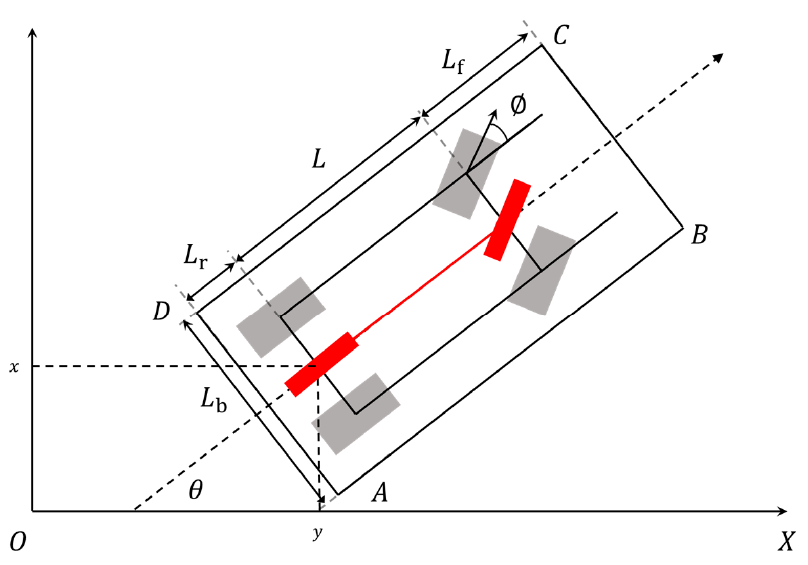
\includegraphics[width=0.6\textwidth]{gambar/bicycle_model.png}
  \caption{Model kinematika kendaraan \parencite{Li2024GaussianPSM}}
  \label{fig:bicyclemodel}
\end{figure}

\emph{Kinematic bicycle model} dapat dianggap valid hanya terbatas pada percepatan lateral $a_y < 0{,}5\mu g$, sehingga model ini hanya akurat pada kecepatan rendah dan jalan datar \parencite{BouGhosn2024ITSC}. Hubungan geometris antara sudut kemudi dan kurvatur lintasan diberikan oleh:

\begin{equation}
  \Phi = \arctan(\kappa \cdot L),
  \label{eq:steering_curvature}
\end{equation}

dengan $\kappa$ adalah kurvatur lintasan dan $L = l_f + l_r$ adalah \emph{wheelbase} kendaraan. Hubungan ini memungkinkan konversi langsung antara kurvatur lintasan yang dihasilkan oleh \emph{planner} trajektori menjadi sudut kemudi yang dapat dieksekusi oleh aktuator kendaraan.

\subsection{\emph{Trajectory Sampling} Berbasis \emph{Circular Arc}}
\label{subsec:arc-fan}

\emph{Trajectory sampling} merupakan metode pemilihan lintasan yang membangkitkan sejumlah kandidat busur lingkaran pada rentang kurvatur yang \emph{feasible} bagi kendaraan, kemudian mengevaluasi setiap kandidat berdasarkan fungsi biaya untuk memilih lintasan optimal. Berbeda dengan \emph{pure pursuit} yang hanya mengevaluasi satu titik \emph{lookahead} dan menghasilkan satu kurvatur, \emph{trajectory sampling} mempertimbangkan banyak alternatif lintasan secara simultan.

\textcite{Li2013AdaptivePreview} mengusulkan metode \emph{roadside sampling} pada \emph{adaptive preview path tracker}. Dalam pendekatan ini, lingkungan jalan lokal direpresentasikan dalam sistem koordinat \emph{body-frame} kendaraan, di mana jalan dideskripsikan melalui tiga kurva: $f_l(x)$ sebagai batas kiri jalan, $f_r(x)$ sebagai batas kanan jalan, dan $f_m(x) = (f_l(x) + f_r(x))/2$ sebagai garis tengah, sebagaimana diilustrasikan pada Gambar \ref{fig:roadside_sampling}. Untuk setiap titik \emph{sampling} $x_i$ di sepanjang sumbu longitudinal, dihitung kurvatur busur lingkaran yang menghubungkan posisi kendaraan ke titik $(x_i, f_m(x_i))$ menggunakan fungsi $\kappa(x_i) = 2y_i/(x_i^2 + y_i^2)$. Algoritma \emph{Find\_Feasible\_Trajectories} memeriksa kelayakan setiap busur berdasarkan batas maksimum kurvatur kendaraan ($|\kappa| \leq \kappa_{max}$) dan ketersediaan rentang kurvatur yang memenuhi batas kiri dan kanan jalan ($\kappa_{l,min} < \kappa_{r,max}$).

\begin{figure}[H]
  \centering
  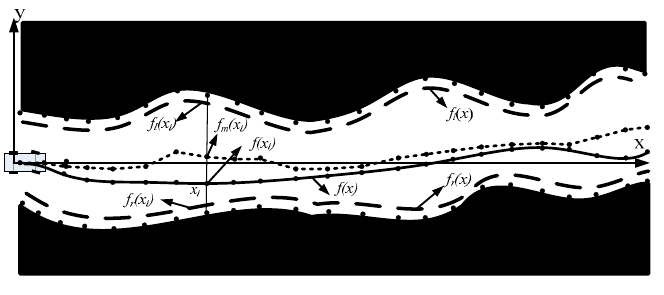
\includegraphics[width=0.8\textwidth]{gambar/local_road_body_frame.png}
  \caption{Representasi lingkungan jalan dalam koordinat \emph{body-frame} kendaraan \parencite{Li2013AdaptivePreview}}
  \label{fig:roadside_sampling}
\end{figure}

Pemilihan trajektori optimal dari himpunan kandidat \emph{feasible} dilakukan melalui fungsi utilitas tiga suku \parencite{Li2013AdaptivePreview}:

\begin{equation}
  i^* = \arg\min_i \left\{ \omega_1 \frac{x_N}{x_N + x_i} + \omega_2 \sum_{m=1}^{i} \frac{|f_d(x_m) - f_m(x_m)|}{s(x_i)}^2 + \omega_3 \, |\kappa(x_i) - \kappa_0|^2 \right\},
  \label{eq:li_utility}
\end{equation}

\noindent dengan $\omega_1$, $\omega_2$, $\omega_3$ adalah bobot masing-masing suku, $x_N$ adalah jarak maksimum lingkungan lokal, $f_d(x)$ adalah lintasan yang diinginkan, $s(x_i)$ adalah panjang busur, dan $\kappa_0$ adalah kurvatur kendaraan saat ini. Suku pertama memprioritaskan jarak pandang yang lebih jauh, suku kedua meminimalkan \emph{cross-track error}, dan suku ketiga menjaga kelancaran perubahan kemudi.

\subsection{Direct LiDAR-Inertial Odometry}
\label{subsec:dlio}

Direct LiDAR-Inertial Odometry (DLIO) merupakan algoritma odometri yang memadukan data \emph{Light Detection and Ranging} (LiDAR) dengan sensor \emph{Inertial Measurement Unit} (IMU) untuk menghasilkan estimasi posisi dan orientasi kendaraan secara \emph{real-time} \parencite{Chen2023DLIO}.
Berbeda dengan metode odometri LiDAR atau odometri LiDAR dan IMU yang memproses titik \emph{point cloud} secara berurutan, DLIO menggunakan pendekatan \emph{continuous-time motion correction} untuk mengoreksi distorsi gerak pada setiap titik \emph{point cloud} LiDAR.
Distorsi ini timbul ketika kendaraan bergerak selama periode akuisisi data dan menjadi signifikan pada manuver agresif atau medan tidak rata.
Hasil koreksi distorsi metode DLIO ditunjukkan pada Gambar \ref{fig:dlio_motion_correction} di mana \emph{point cloud} yang awalnya terdistorsi menjadi lebih rapi setelah dikoreksi.

\begin{figure}[H]
  \centering
  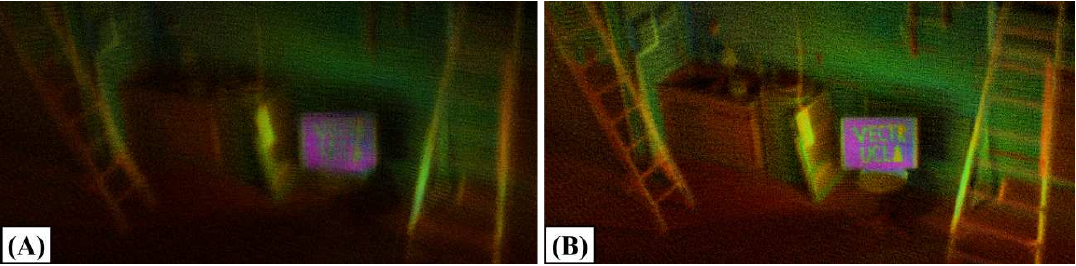
\includegraphics[width=0.8\textwidth]{gambar/deskew.png}
  \caption{Perbandingan \emph{point cloud} LiDAR sebelum (A) dan sesudah (B) koreksi distorsi gerak menggunakan DLIO \parencite{Chen2023DLIO}}
  \label{fig:dlio_motion_correction}
\end{figure}

Algoritma ini menggunakan \emph{nonlinear geometric observer} yang memberikan estimasi \emph{state} dengan jaminan konvergensi kuat, yang digunakan untuk menginisialisasi integrasi IMU yang sensitif sehingga memungkinkan koreksi distorsi titik per titik secara cepat dan dapat diparalelkan.
Validasi data DLIO dilakukan pada lima segmen pengujian dengan total panjang lintasan lebih dari 6 km.
DLIO dalam konfigurasi \emph{continuous-time motion correction} mencatatkan RMSE terendah mencapai RMSE 0,0612 m pada lintasan sepanjang 97,2 m dan 0,32 m pada jarak 3063,42 m.
Meskipun demikian, perlu dicatat bahwa DLIO tetap memiliki galat akumulatif sendiri karena berbasis odometri LiDAR-IMU.

\subsection{Dynamic Window Approach}
\label{subsec:dwa}

\emph{Dynamic Window Approach} (DWA) merupakan metode perencanaan gerak lokal yang membangkitkan kandidat lintasan dalam ruang kecepatan (\emph{velocity space}) yang dapat dilalui bagi kendaraan \parencite{Cao2025SOADWA}. Ruang pencarian dibatasi oleh \emph{dynamic window} yaitu himpunan pasangan kecepatan linier dan sudut $(v, \omega)$ yang dapat dicapai kendaraan dalam periode waktu tertentu dengan mempertimbangkan keterbatasan akselerasi.

Setiap kandidat lintasan dievaluasi menggunakan fungsi objektif yang terdiri dari tiga komponen:

\begin{equation}
G(v, \omega) = \alpha \cdot \text{heading}(v, \omega) + \beta \cdot \text{dist}(v, \omega) + \gamma \cdot \text{vel}(v, \omega),
\label{eq:dwa_original}
\end{equation}

dengan $\alpha$, $\beta$, dan $\gamma$ adalah bobot masing-masing komponen. \emph{Heading} mengukur keselarasan arah gerak terhadap titik tujuan, \emph{dist} mengukur jarak terdekat ke \emph{obstacle} sepanjang lintasan, dan \emph{vel} mendorong kendaraan bergerak maju secepat mungkin \parencite{Cao2025SOADWA}. Kandidat dengan nilai $G$ tertinggi dipilih sebagai lintasan optimal.

\subsection{Dijkstra untuk Perencanaan Rute Global}
\label{subsec:global-planning}

Algoritma Dijkstra adalah metode untuk mencari rute terpendek dari satu titik ke titik lain dalam jaringan jalan yang direpresentasikan sebagai graf \parencite{Cormen2001}. Graf terdiri dari simpul yang mewakili persimpangan atau segmen jalan, dan sisi yang mewakili hubungan antar segmen dengan bobot berupa jarak atau jumlah titik antara yang ditunjukkan pada Gambar \ref{fig:dijkstra_graph}.
Algoritma ini menggunakan pendekatan \emph{greedy} untuk menemukan jalur terpendek dengan memanfaatkan struktur data \emph{priority queue} untuk menyimpan simpul yang akan dieksplorasi berikutnya.

\begin{figure}[H]
  \centering
  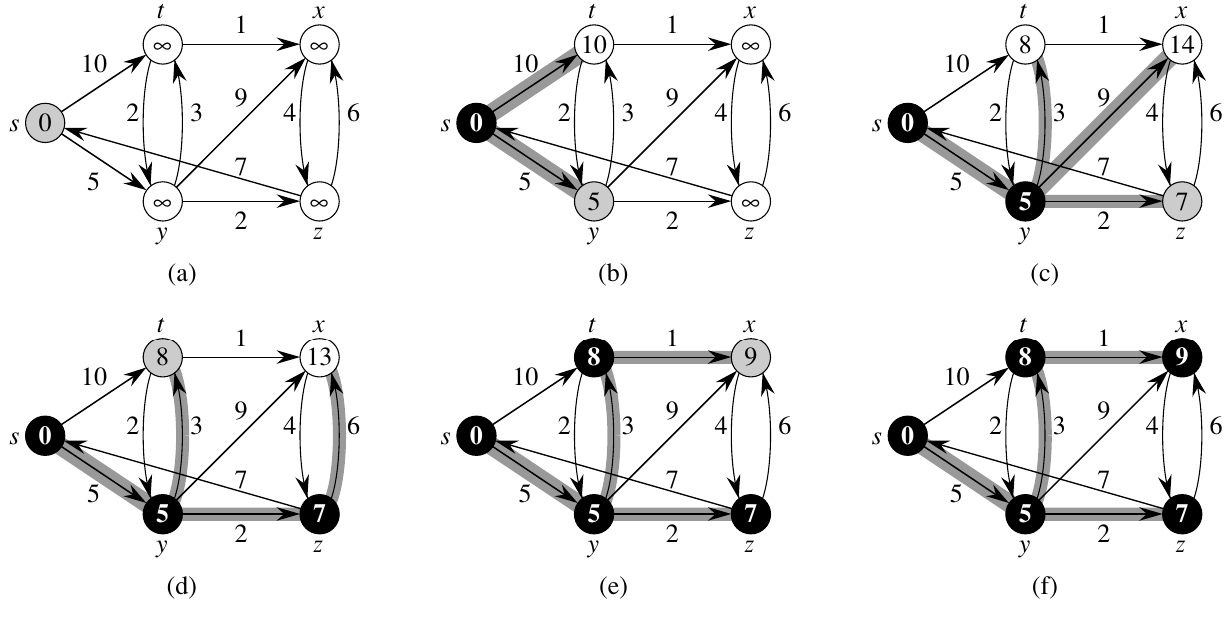
\includegraphics[width=0.8\textwidth]{gambar/dijkstra.png}
  \caption{Contoh graf untuk perencanaan rute global menggunakan algoritma Dijkstra \parencite{Cormen2001}}
  \label{fig:dijkstra_graph}
\end{figure}

Algoritma bekerja secara bertahap yang dimulai dari simpul awal, algoritma mengunjungi simpul terdekat yang belum dikunjungi, kemudian memperbarui jarak ke simpul-simpul tetangganya jika ditemukan rute yang lebih pendek.
Langkah ini diulang hingga semua simpul dikunjungi dan jarak terpendek ke seluruh simpul diketahui. Algoritma Dijkstra menjamin hasil optimal selama tidak ada sisi berbobot negatif, dengan waktu komputasi yang efisien untuk graf berskala ratusan simpul \parencite{Cormen2001}.